\documentclass{procDDs}
                                                  % load packages only if necessary

\title{Experimental Study of Diffraction by a Thin Cone}

\author{\textbf{Belous A.A.}, Korolkov A.I., Shanin A.V.}% List of authors with the
{Faculty of Physics, Lomonosov Moscow State University, Russia}                 % same affiliation,
                                                  % lecturer given in bold
{artem.belous@gmail.com}                                   % e-mail of lecturer
%
%                                                 % it is important not to have
%                                                 % blank lines between the
%                                                 % \author and \coauthor
%
%\coauthor{Name I. Coauthor}                       % Co-author(s) with
%{Institute, University, Country}                  % another affiliation
%{coauthor@e.mail }                                               % use such line
                                                  % if e-mail none available

\begin {document}

\maketitle

\index{Belous, A.A.}                              % write this for each author
\index{Korolkov, A.I.}                              % to generate the index
\index{Shanin, A.V.}                             %

\begin{abstract}   
   A problem of diffraction by elongated body of revolution is studied. A direct diffraction experiment is used to measure the diffracted field on the surface of a thin cone. The experiment is performed using MLS (Maximum Length Sequence) method. The incident field falls from different directions. The wavelengths are small comparatively to the length of the cone. A boundary integral equation is used to describe the field theoretically. The integral equation is solved numerically by iterations. The results of the experiment are calculated with the results of the calculation.
\end{abstract}

\section{Introduction}

   Diffraction by a thin cone  attracts considerable attention of researchers. Several different approaches exist to developing both asymptotics of the diffracted field and the diffracted field itself. First, there is a traditional asymptotic approach based on ray representation \cite{Popov}. Second, there is an approach based on the parabolic equation method \cite{Andronov}. Third, there is an approach based on the boundary integral equation method for the parabolic equation in Cartezian coordinates \cite{Shanin1}. Also, there is an approach based on the Smyshlyaev's formula \cite{Smychlyaev}, and an approach based on Kontorovich-Lebedev  integral representation \cite{Lyalinov}. All these methods are mathematically complicated, and the question about which one works better is still open.
   
   In this work, a direct diffraction experiment is used to measure the field diffracted by a cone. The experiment is performed using MLS technique \cite{Shanin}. We put our receiver to the surface of the cone. After that the cone is irradiated by a point source from different directions so that the receiver is enlightened or shadowed. The parabolic equation of diffraction theory is used as the governing equation. The boundary integral equation developed in \cite{Shanin_parabolic} is used to calculate the diffracted field being compared to the results of the experiment. The equation is of Volterra type, so it is solved by iterations.
   

\section{Experiment}

\subsection{Description}
A narrow (the angle is $\alpha = 5.5 ^{\circ}$) duralumin cone (see Fig.~\ref{cone}) is hanged in free space. A point-sized microphone is placed on the surface of the cone. The cone is irradiated by a point source from different directions so the receiver can be shadowed or enlightened (see Fig.~\ref{exp_scheme}). A miniature armature Knowles driver is used as a source and a well-calibrated no-name microphone is used as a receiver. 

\begin{figure}[t!]\centering
	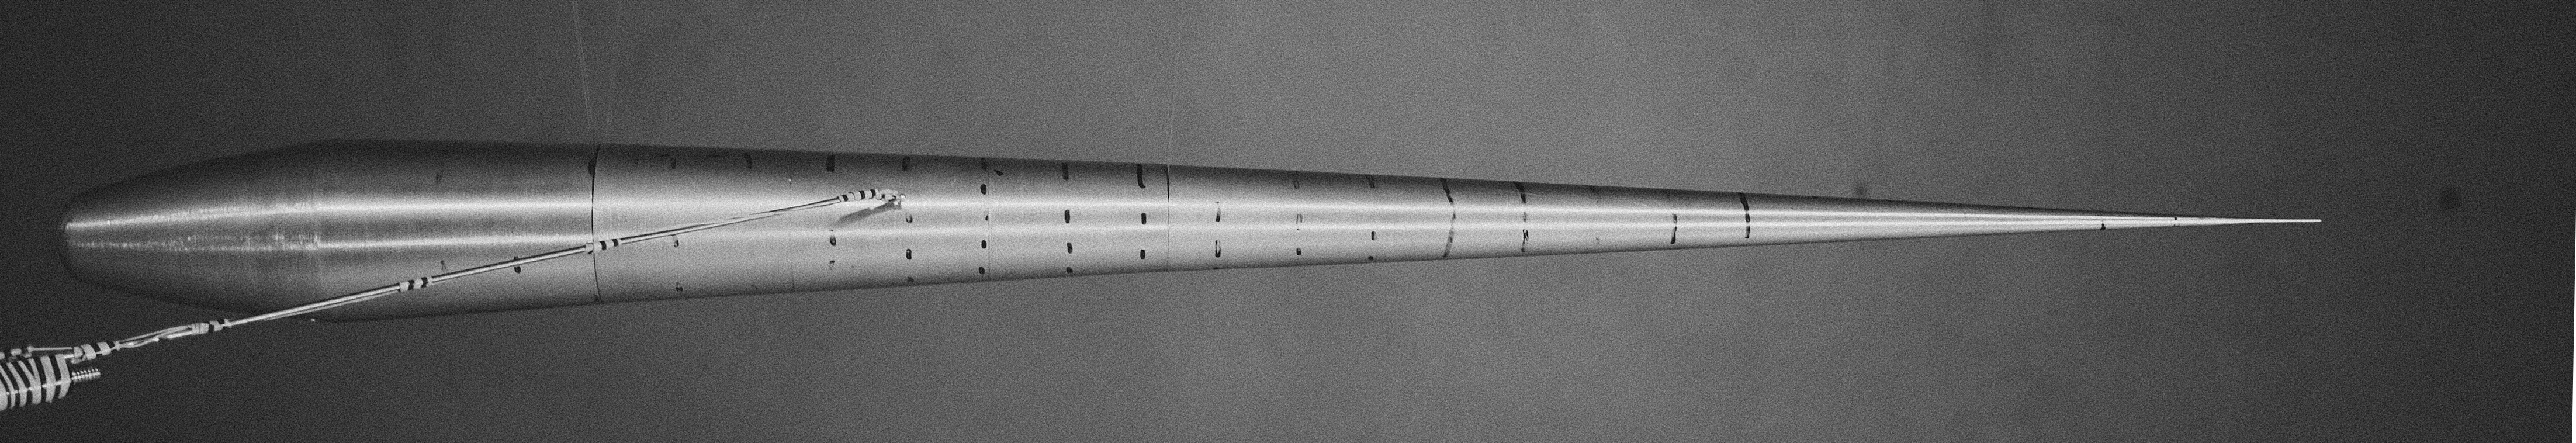
\includegraphics[width=.5\textwidth]{cone.jpeg}
	\caption{Photo of the duralumin cone with the mic on its surface.}\label{cone}
\end{figure}


To conduct the experiment, MLS method is used \cite{Shanin}. The cone is irradiated by a pseudo-random signal and then impulse response of the acoustical path is calculated through calculating correlation of the MLS signal with the output signal.

\begin{figure}[t!]\centering
	\includegraphics[width=.5\textwidth]{experiment.eps}
	\caption{Experiment scheme, view from above.}\label{exp_scheme}
\end{figure}

The input MLS signal is correlated with the measured signal (see Fig.~\ref{processing}) and impulse response is calculated. The procedure is identical to that described in \cite{Shanin}. From impulse response a region of interest corresponding to diffraction by the cone is cropped. After that the frequency dependence of this region is calculated and compared to theory.

\begin{figure}[t!]\centering
	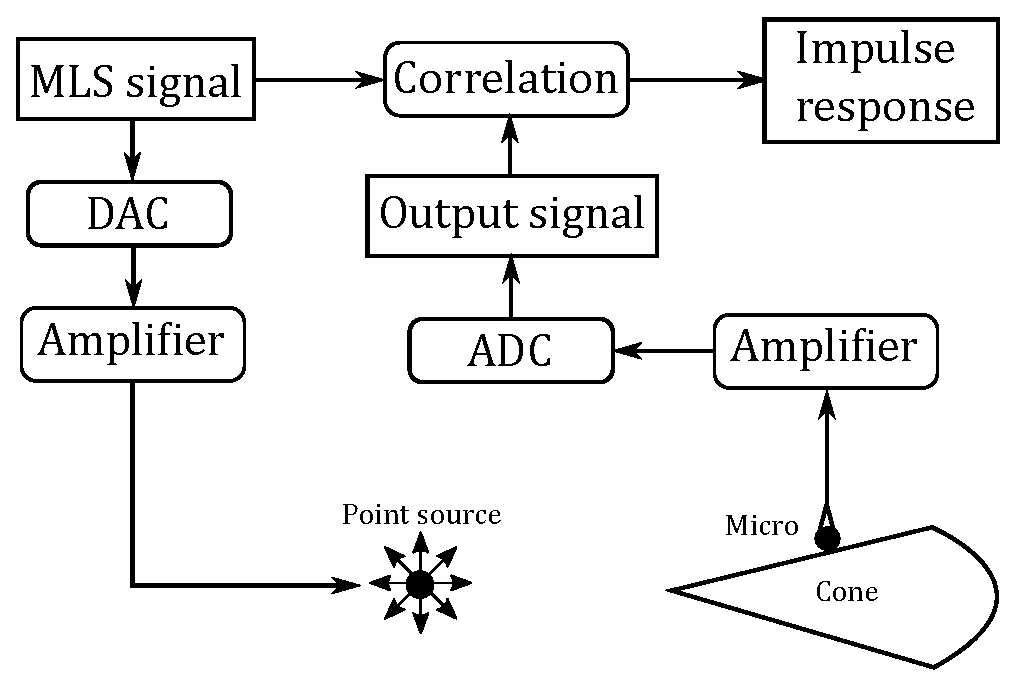
\includegraphics[width=.48\textwidth]{processing.eps}
	\caption{Experimental data processing scheme.}\label{processing}
\end{figure}


\section{Theoretical description}

\subsection{Problem statement}

The acoustical field is described using Helmholtz equation:

\begin{equation}\label{helm}                     
\Delta \tilde{u} + k^2 \tilde{u} = 0.                                         
\end{equation}

Our cone is very narrow (its vertex angle is much smaller than 1 radian) so most of the waves are going to be scattered under small angles. This means that the parabolic equation of diffraction theory can be used to describe the field on the surface of the cone so the field on the surface of the cone can be represented as follows:

\begin{equation}\label{parab_field}                     
\tilde{u}(x,r,\varphi)=\exp\left\lbrace ikx \right\rbrace u(x,r,\varphi),                                         
\end{equation}
where $u$ is a slow function of $x$, compared to the exponential factor. Substituting (\ref{parab_field}) in (\ref{helm}) and neglecting the term with the second $x$-derivative, get the approximate equation for $u$:

\begin{equation}\label{parab_eqn}                     
\left( \frac{\partial}{\partial x} + \frac{1}{2ik} \Delta_\perp \right) u = 0,                                 
\end{equation}
which is the parabolic equation of the diffraction theory (PETD).

As we are using a point source, its field will be equal to Green's function of the parabolic equation. Let us denote the points of space by $\vec{r} = (x, r, \varphi)$ and the point source be located at $\vec{r_s} = (x_s, r_s, \varphi_s)$. Thus the field of the source will be the solution of

\begin{equation}\label{greens_eqn}                     
\left(  \frac{\partial}{\partial x} + \frac{1}{2ik} \Delta_\perp \right) g(\vec{r}, \vec{r_s}) = \delta(\vec{r} - \vec{r_s}),                                 
\end{equation}
where the operator in the left part acts on the components of $\vec{r}$, $\delta$ is the Dirac's delta-function. The solution should obey the initial condition, i. e. it should be equal to zero for $x < x_s$.

One can check that the Green's function for $x > x_s$ will be

\begin{equation}\label{greens_sol}                     
g(\vec{r}, \vec{r_s}) = \frac{k}{2\pi i (x-x_s)} \exp \left[   \frac{ik}{2} \frac{(\Delta r)^2}{x-x_s}\right],
\end{equation}
where $\Delta r$ is the distance between the projections of $\vec{r}$ and $\vec{r_s}$ onto the transversal plane:

\begin{equation}\label{delta_r}                     
(\Delta r)^2 = r^2 + r_s^2 - 2r r_s \cos(\varphi - \varphi_s).
\end{equation}


\subsection{Calculating the diffracted field}

In \cite{Shanin_parabolic} a boundary equation is derived for the field diffracted by a body of revolution. The equation is applied to the bodies having their curvature dependent on $x$ like $r = f(x)$. We are going to apply the results of \cite{Shanin_parabolic} for our conical case.

Let $U$ be the full field on the surface, $U^{\text{in}}$ be the incident field on the surface. Both of these fields depend only on $x$ and $\varphi$. If $x_*, \varphi_*$ are coordinates of the observation point, $X$ is such that $f(x<X) = 0$ (for the case of the cone $X$ is the coordinate of its vertex), then

\begin{multline}\label{int_eq} 
U(x_*, \varphi_*) = \int_{0}^{2\pi}\int_{X}^{x_*} K(x_*, \varphi_*, x, \varphi) U(x, \varphi) dx d\varphi \\
+ 2U^{\text{in}}(x_*, \varphi_*),
\end{multline}

\begin{multline} \label{int_ker}                   
K(x_*, \varphi_*, x, \varphi) = \frac{ikf(x)}{2\pi} \times \\
\left[ \frac{\dot{f}(x)}{x_* - x} +\frac{f(x) - f(x_*) \cos(\varphi - \varphi_*)}{(x_* - x)^2}\right] \times \\
\exp \left\lbrace  \frac{ik}{2}  \frac{f^2(x_*) + f^2(x) - 2f(x_*) f(x) \cos(\varphi - \varphi_*)}{x_* - x} \right\rbrace,
\end{multline}

For our case $f(x)$ is a linear function of $x$, $r = f(x) = \tan(\alpha/2) x \approx x \alpha/2 $, where $\alpha$ is the angle at the vertex of our cone.

Note that equation (\ref{int_eq}) is of Volterra type with respect to variable $x$, and is of difference kernel type with respect to the variable $\varphi$.
This means that it can be solved using iterations with respect to $x$.

Let us discretize the field $U(x, \varphi)$. We need to define linear shape functions $N_i(x)$ such that:

\begin{equation}
N_i(x) = 
\begin{cases}
&1, \quad x=x_i,\\
&0, \quad x\neq x_i.
\end{cases}
\end{equation}

Then 

\begin{equation} \label{discr}
U(x, \varphi) = \sum_{i} U_i N_i(x).
\end{equation}

We substitute (\ref{discr}) to (\ref{int_eq}) and get

\begin{multline} \label{final_eq}
U(x_*, \varphi_*) \approx \\
\sum_{i} U_i \int_{0}^{2\pi} \int_{X}^{x_*} K(x_*, \varphi_*, x, \varphi) N_i(x) dx d\varphi \\
+ 2U^{\text{in}}(x_*, \varphi_*).
\end{multline}

Now, (\ref{int_eq}) becomes a discretized matrix equation and $K(x_*, x)$ becomes a lower-triangle matrix. $K(x_*, x)$ has a pole at $x = x_*$ we need to deal with to calculate the integral in (\ref{final_eq}). To do this we slightly ($\varepsilon \ll X$) shift the integration contour to the upper complex half-plane $x \rightarrow x + i\varepsilon$, see Fig.~\ref{contour}. 

\begin{figure}[t!]\centering
	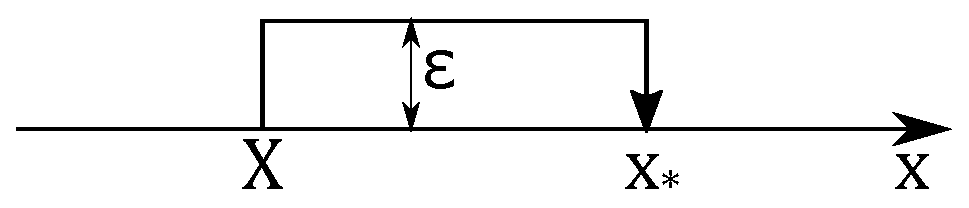
\includegraphics[width=.4\textwidth]{contour.eps}
	\caption{Integration contour for (\ref{contour}).}\label{contour}
\end{figure}

Equation (\ref{final_eq}) can be solved by iterations with respect to $x$:

\begin{align}                       % key is any name used
& U(x) = \sum_{n=0}^{\infty} U^{\text{(n)}}(x) ,\notag\\
& U^{(0)}(x) = 2U^{\text{in}}(x),\label{key3}\\
& U^{(n+1)}(x_*) = \int_X^{x_*} K(x_*, x) U^{\text{(n)}}(x) dx, \quad n>0 \notag 
\end{align}

We calculate the solution for each frequency $\omega$ and finally we get $U(\omega)$ for the field in observation point (see Fig.~\ref{exp_scheme}). 


\section{Experimental results and modeling}

\subsection{Axial incidence}

For axial incidence, one can notice that the field fades like $1/x$ which is just fading due to the spherical front of the incident field. This means that the incident field doesn't feel the presence of the obstacle and thus is not diffracted.



\begin{figure}[t!]\centering
	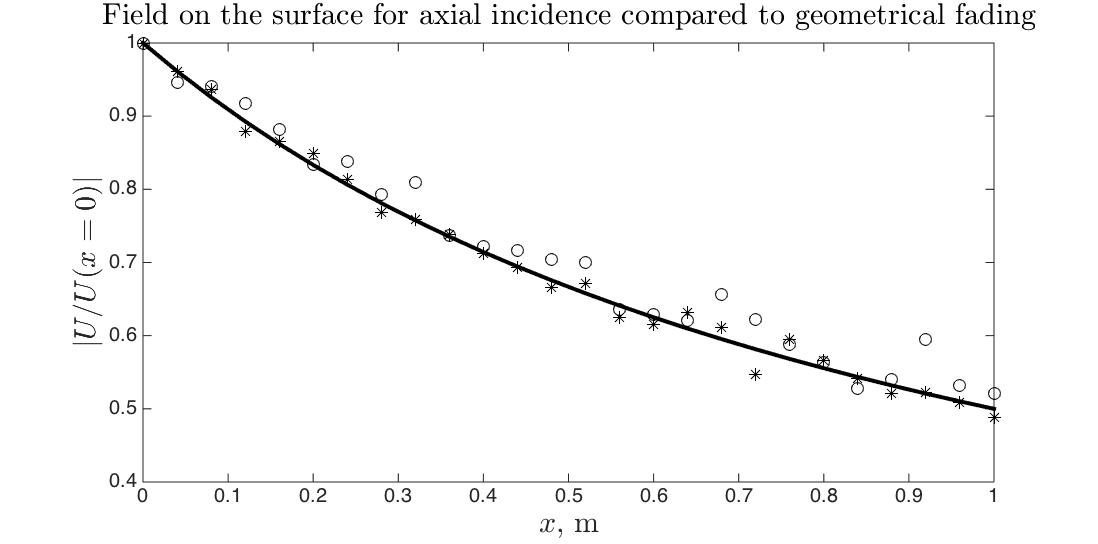
\includegraphics[width=.5\textwidth]{axial.jpg}
	\caption{Measured field for different $x$ for $f = 2000$ Hz (circles) and for $f = 3000$ Hz (stars) compared to geometrical fading $\sim 1/(x+1)$.}\label{axial}
\end{figure}

\textbf{I have difficulties with this part. The length of the Fresnel zone on the surface of the cone for 1000 Hz is approximately 17 cm, so there are several of them on our cone. I don't know how to explain the absence of diffraction under axial incidence.}

\subsection{Non-axial incidence}

The experimental results are compared to modeling results for $y_s = -0.5, -0.4,..., 0.4, 0.5$ (see Fig.~\ref{y01}, ~\ref{y03}, ~\ref{y05}). The field in the figures is represented in terms of the incident field, 1 corresponds to $U^{\text{in}}(x)$.

\begin{figure}[t!]\centering
	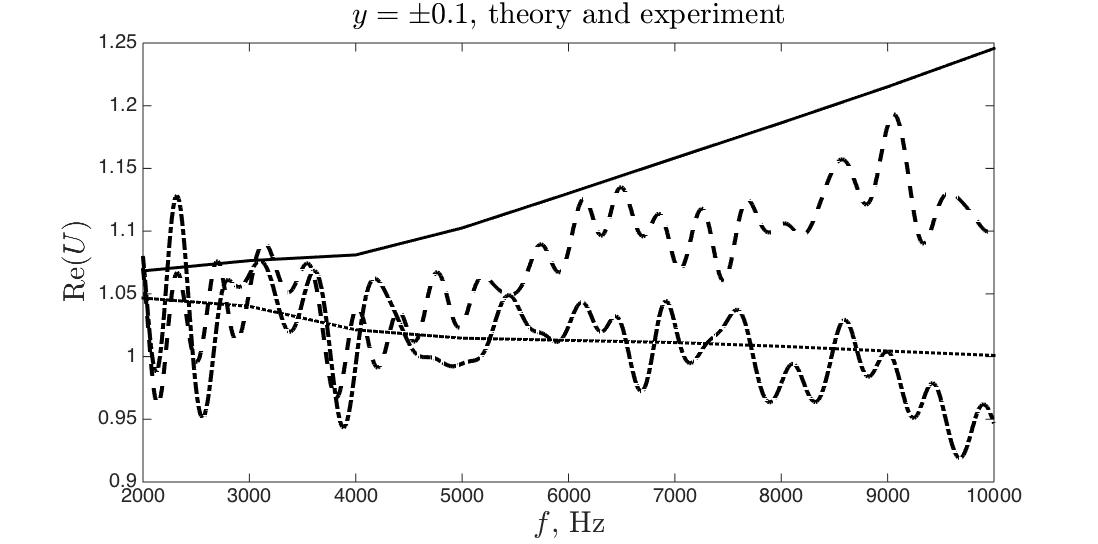
\includegraphics[width=.51\textwidth]{y01.jpg}
	\caption{Comparison of experiment and theory for $y = \pm 0.1$. Theory (solid line) and experiment (dashed line) for $y = -0.1$, theory (dotted line) and experiment (dash-dotted line) for $y = 0.1$.}\label{y01}
\end{figure}

\begin{figure}[t!]\centering
	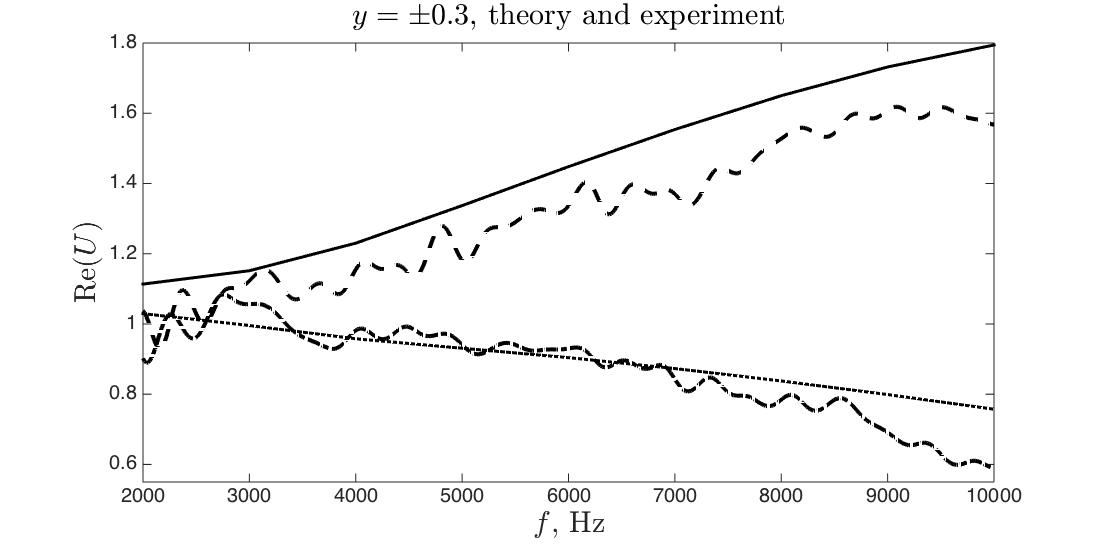
\includegraphics[width=.51\textwidth]{y03.jpg}
	\caption{Comparison of experiment and theory for $y = \pm 0.3$. Theory (solid line) and experiment (dashed line) for $y = -0.3$, theory (dotted line) and experiment (dash-dotted line) for $y = 0.3$.}\label{y03}
\end{figure}

\begin{figure}[t!]\centering
	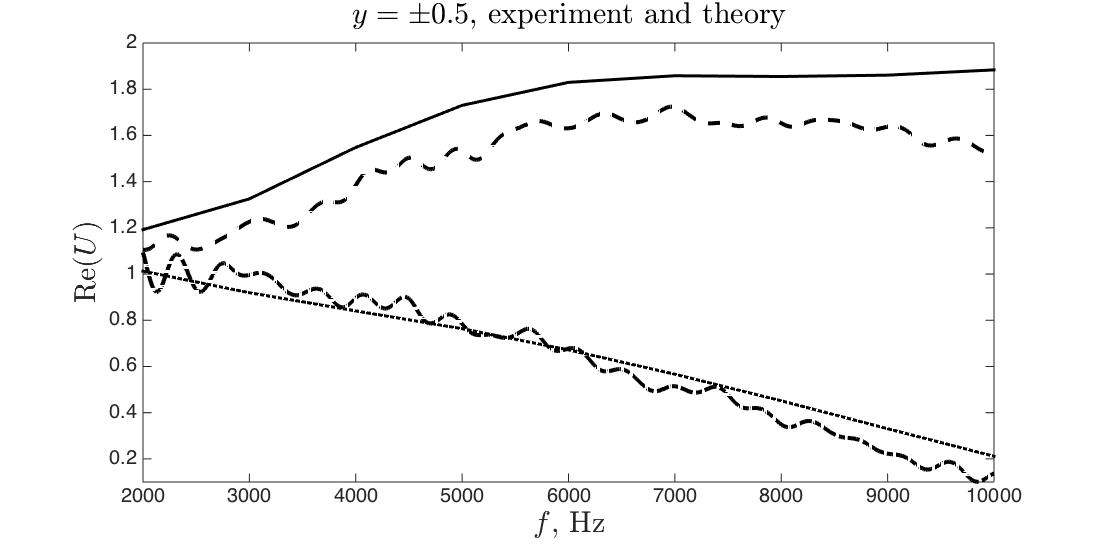
\includegraphics[width=.51\textwidth]{y05.jpg}
	\caption{Comparison of experiment and theory for $y = \pm 0.5$. Theory (solid line) and experiment (dashed line) for $y = -0.5$, theory (dotted line) and experiment (dash-dotted line) for $y = 0.5$.}\label{y05}
\end{figure}

The experimental results highly depend on the phase shift which is technically the distance between the point source and the microphone. The distances in our experiments were measured with error about $\pm 1$ cm, so we attenuated the phase shift during the calculations by hand within $\Delta = 1$ cm via multiplying the field by $\exp(ik\Delta)$.

What we see for the cases of negative $y$ when the source becomes enlightened is that the field tends to 2. This is pretty much what we expect because the field should show the reflection from a hard wall and thus be the incident field doubled. For the case of positive $y$ the field on the mic is that transmitted along the cone. Its amplitude fades while the frequency grows as the high-frequency field feels the obstacle.

\section{Conclusion}

In this work, a direct diffraction experiment was held on diffraction by a narrow cone with the use of a point source. The results of the experiment for axial incidence show that there is almost no diffraction due to a big longitudinal size of the Fresnel zone along the cone surface. For non-axial incidence the results agree with the diffraction theory in parabolic approximation. The theoretical results were calculated using iterations.


\iffalse 

Body of subsection.

Numbered formula should be written as
\begin{equation}\label{key}                       % key is any name used
a+b=2.                                         % to refer to the formula
\end{equation}

The reference to such an equation should be as (\ref{key}).

A few formulae:
\begin{gather}                       % key is any name used
a+b=2,\label{key1}\\
c+d=3.\label{key2}
\end{gather}


Aligned formulae:
\begin{align}                       % key is any name used
A={}&\int_0^1f(x)\mathrm{d}x,\notag\\
&{}+a+b+c,\label{key3}\\
B={}&3.\label{key4}
\end{align}

A long formula:
\begin{multline}
D=a+b+c+e+\sum_{n=1}^\infty t_n\\
+f+\int_0^1g(x)\mathrm{d}x+q+h+y^2\\
-r-s-\sin(w).
\end{multline}
 
% See http://mirror.ctan.org/macros/latex/required/amslatex/math/amsldoc.pdf
% for more examples of AMS-LaTeX commands.
 
Citations are written as \cite{paper1}.           % paper1 is the name from
                                                  % \bibitem commands below
Fig.~\ref{fig1} shows handling of figures.

%\begin{figure}[t!]\centering
%  \includegraphics[width=.43\textwidth]{Test_fig.eps}
%  \caption{This is test figure}\label{fig1}
%\end{figure}



\section*{Acknowledgements}

Put acknowledgements in the last section, please do not use footnotes for that.

%  citations should be arranged by order of appearance
\fi
\begin {thebibliography}{9}
	
\bibitem{Popov} Popov A., Ladyzhensky A., Khozioski S., 2009, Uniform Asymptotics of the Wave Diffracted by a Cone of Arbitrary Cross Section,  \emph{Russ. J. Math. Phys.}. Vol. \textbf{16}, no. \textbf{2}, p. 296-–299.
	
\bibitem{Andronov} Andronov I. V., 2011, Diffraction by a Strongly Elongated Body of Revolution, \emph{Acoust. Phys.} . Vol. \textbf{57}, p. 147–-152.
	
\bibitem{Shanin1} A.\,V\;Shanin, A.\,I\;Korolkov, 2017,  Diffraction by a thin cone in the parabolic approximation. Method of the boundary integral equation, \emph{ICEAA Proceedings 2017}, DOI: 10.1109/ICEAA.2017.8065342
	
\bibitem{Smychlyaev} V.\,M\;Babich, D.\,B\;Dement'ev, B.\,A\; Samokish, V.\,P\; Smychlyaev, 2000, On evaluation of the diffraction coefficient for arbitrary "nonsingular" directions of a smooth convex cone, \emph{SIAM J. Appl. Math}, Vol. \textbf{60}, no. \textbf{2}, p. 536--573.
	
\bibitem{Lyalinov} Lyalinov M. A., Zhu N. Y., 2007, Acoustic scattering by a circular semitransparent conical surface, \emph{J. Eng. Math.}. Vol. \textbf{59}, no. \textbf{4}, p. 385--398.
	
\bibitem{Shanin} Shanin A. V., Valyaev V. Yu., 2011, Maximum length sequence method in diffraction experiment, \emph{Acoustical Physics}. Vol \textbf{57}, no. \textbf{3}, p. 420--425.

\bibitem{Shanin_parabolic} Shanin A. V., Korolkov A.I., 2018, Diffraction by an elongated body of revolution. A boundary integral equation based on the parabolic equation, \emph{arxiv.org} arXiv:1704.08857v1.

\end{thebibliography}

\end {document}
